\shorttitle{Introduction}
\section{Introduction}

With the outstanding financial investment of the Jacobs Foundation
in the International University Bremen (IUB)\footnote{Jacobs
University as of Spring 2007}  on October 31, 2006, the future
perspective of the University and in particular the School of
Engineering and Science is on steady and foreseeable grounds. This,
and the advent of the new president Professor Dr. Dr. h.c. mult.
Joachim Treusch, who formally took office by July 1, 2006,
eventually resulted in a reformulation of the key mission and the
main research objectives of the university. The main scientific
activities of the School can be considered to be perfectly
consistent with the new objectives.

\subsection{The Mission}

The International University Bremen has been designed and developed
as an international research university using the anglo-saxon
template, and incorporating the European Bologna Process into its
teaching model. The main mission is to academically educate bright
young people, irrespective of their nationality, religion, sex, race
and financial conditions, in order to prepare them for future
leading roles in our globalized world. Thus, the University is
designed to provide significant contributions towards a peaceful,
and sustainable development of mankind. As a campus university where
students from more than 80 nations live and learn together in
colleges, intercultural understanding and collaboration in daily
life is trained as a byproduct of the university education.

\null
 Research and teaching are closely interwoven and pursued on the same high level
 taking
into account the requirements of practical life in enterprises and
industry. Interdisciplinarity constitutes the key concept. Research
at the International University Bremen aims at delivering key
contributions towards the main challenges of mankind, namely
\newpage
\begin{myitemize}
\item   energy and materials
\item  water and food
\item   health
\item "Bildung" and communication
\item peace and conflict management.
\end{myitemize}


\null
 The School of Engineering and Science contributes with its
activities mainly towards the former three of these, although its
strong electrical engineering faculty addresses technological issues
that are closely related to the latter two.

The scientific objectives of the International University Bremen
concentrate in five
broad areas, namely \\

\begin{myitemize}
\item bio-geo-marine resources - from molecules towards technologies
\item  modeling of complex systems - computer simulation, visualization, networks and management
\item changing societies, cultures, and institutions -  aspects of globalization
\item   Asia and Europe - historical,
psychological and cultural perspectives
\item productive adult development \item "Bildung" and work.
\end{myitemize}


\null
 The five research fields of the School of Engineering and
Science that have been emerging during the founding years contribute
towards the first two of these: Projects within "Information and
Communication Technologies" are directly related to the second
research area. Topics addressed by IUB's "Life Sciences" and
"Geosciences and Astrophysics"  contribute to the first as well as
to the second area. "Nanoscience and Material Research" and
"Mathematics and Theoretical Physics" establish the scientific
backbones of the above. These provide important scientific tools and
the key methods for successfully tackling questions at the
interfaces between the conventional disciplines.

\newpage
 The latter, namely science across disciplinary boarders is
indeed the outstanding - if not the main - trademark of research and
development,  and teaching at the  School of Engineering and
Science.


\subsection{Factual Development During the Founding Period}

\subsubsection{Students}
During the course of the past founding years, the School of
Engineering and Science has been showing remarkable growth, in
quantity as well as in quality. The number of undergraduate
students, starting in 2001 with 67 has now reached its preliminary
saturation at 381 students (Fig.~\ref{fig:students}). Basically this
is dictated by the number of college places and the fact that
according to planning 2/3 of the total number of students can be
admitted to programs of the School. There are now 12 undergraduate
programs of which 10 are formally accredited.


In 2004, for the first time a significant number (48) of graduate
students were admitted to the graduate programs of the School. Since
then, the number of graduate students has been growing to an
impressive total of 223 out of which 142 are PHD-students
(Fig.~\ref{fig:students}). By now, the School has successfully
established seven graduate programs on the master's level.

\begin{figure}[ht]
  \begin{center}
   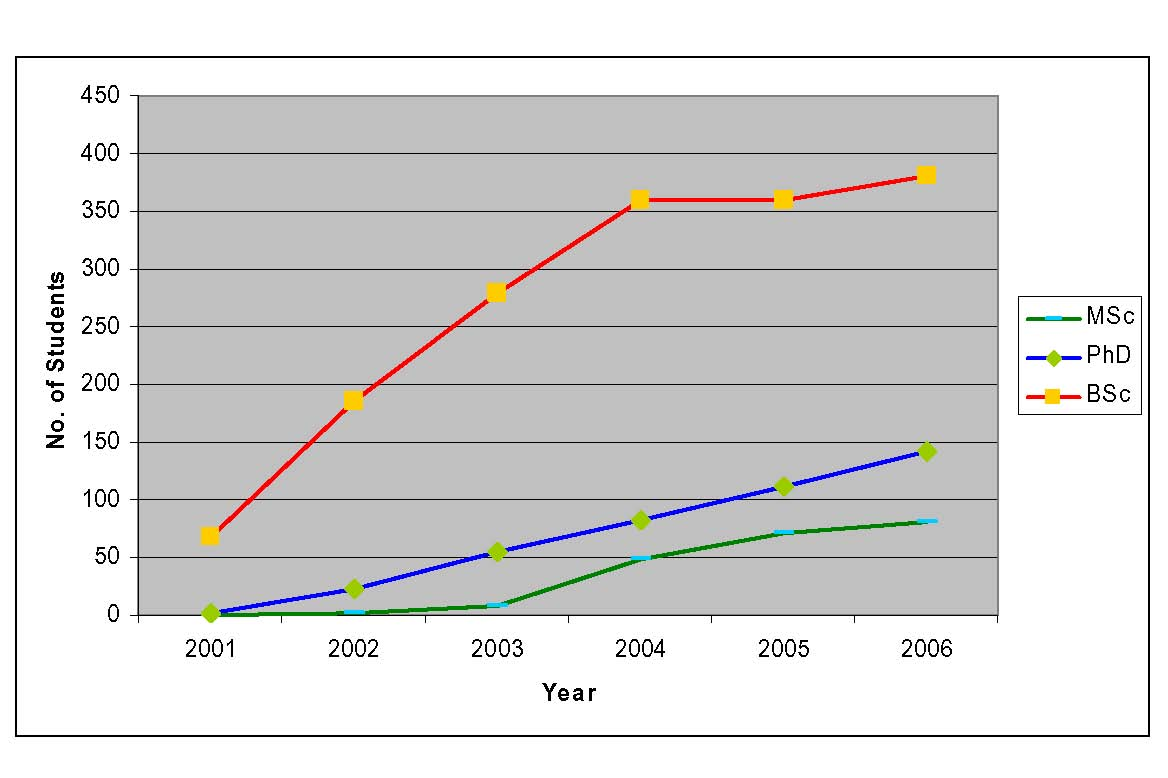
\includegraphics[width=\hsize]{Students.jpg}
   \end{center}
\caption{Temporal Development of Number of Students in the School of
Engineering and Science \label{fig:students}}
\end{figure}

\label{students}

\subsubsection{Publications}

During the founding period, the scientific output of the School,
measured in terms of the number of publications, has been growing
from initially 144 to 389 in 2006, after an intermediate decrease in
2004 which can be understood by having in mind that 2004 has been
the year during which the main research laboratories have been
planned and constructed (Fig.~\ref{fig:publications}). The last of
the laboratories (the Lab II laboratory) has been finished in 2005.

\begin{figure}[ht]
  \begin{center}
   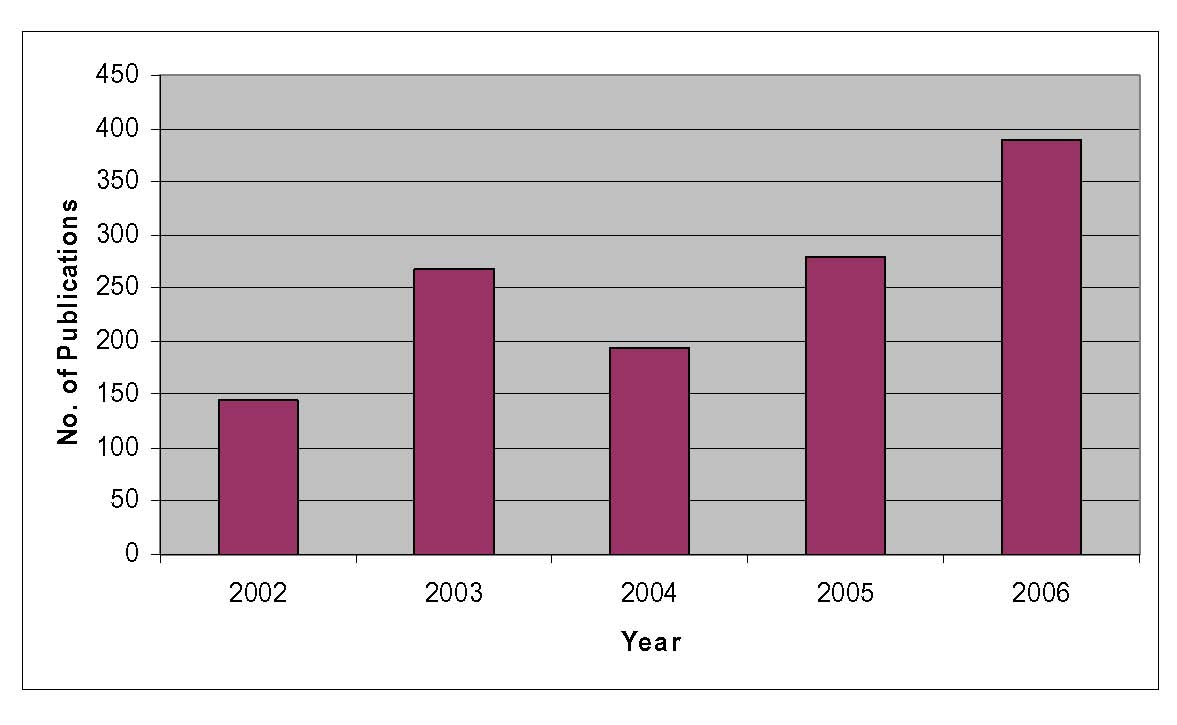
\includegraphics[width=\hsize]{Publications.jpg}
   \end{center}
 \caption{Number of Peer-reviewed Articles, Conference Proceedings, Articles in Encycl./Handbooks,
 Monographs/Books, Editor-ship, and Contribution in Ed. Volumes
 \label{fig:publications}}
\end{figure}


\subsubsection{Grants}
The development of third party funding is summarized in
Fig.~\ref{fig:grants1} and Fig~\ref{fig:grants2}. Revenues from
Research grants have reached a total of more than 4.000.000 EURO in
2006 which implies an average revenue per professor of 82.000 EURO.

\begin{figure}[ht]
  \begin{center}
   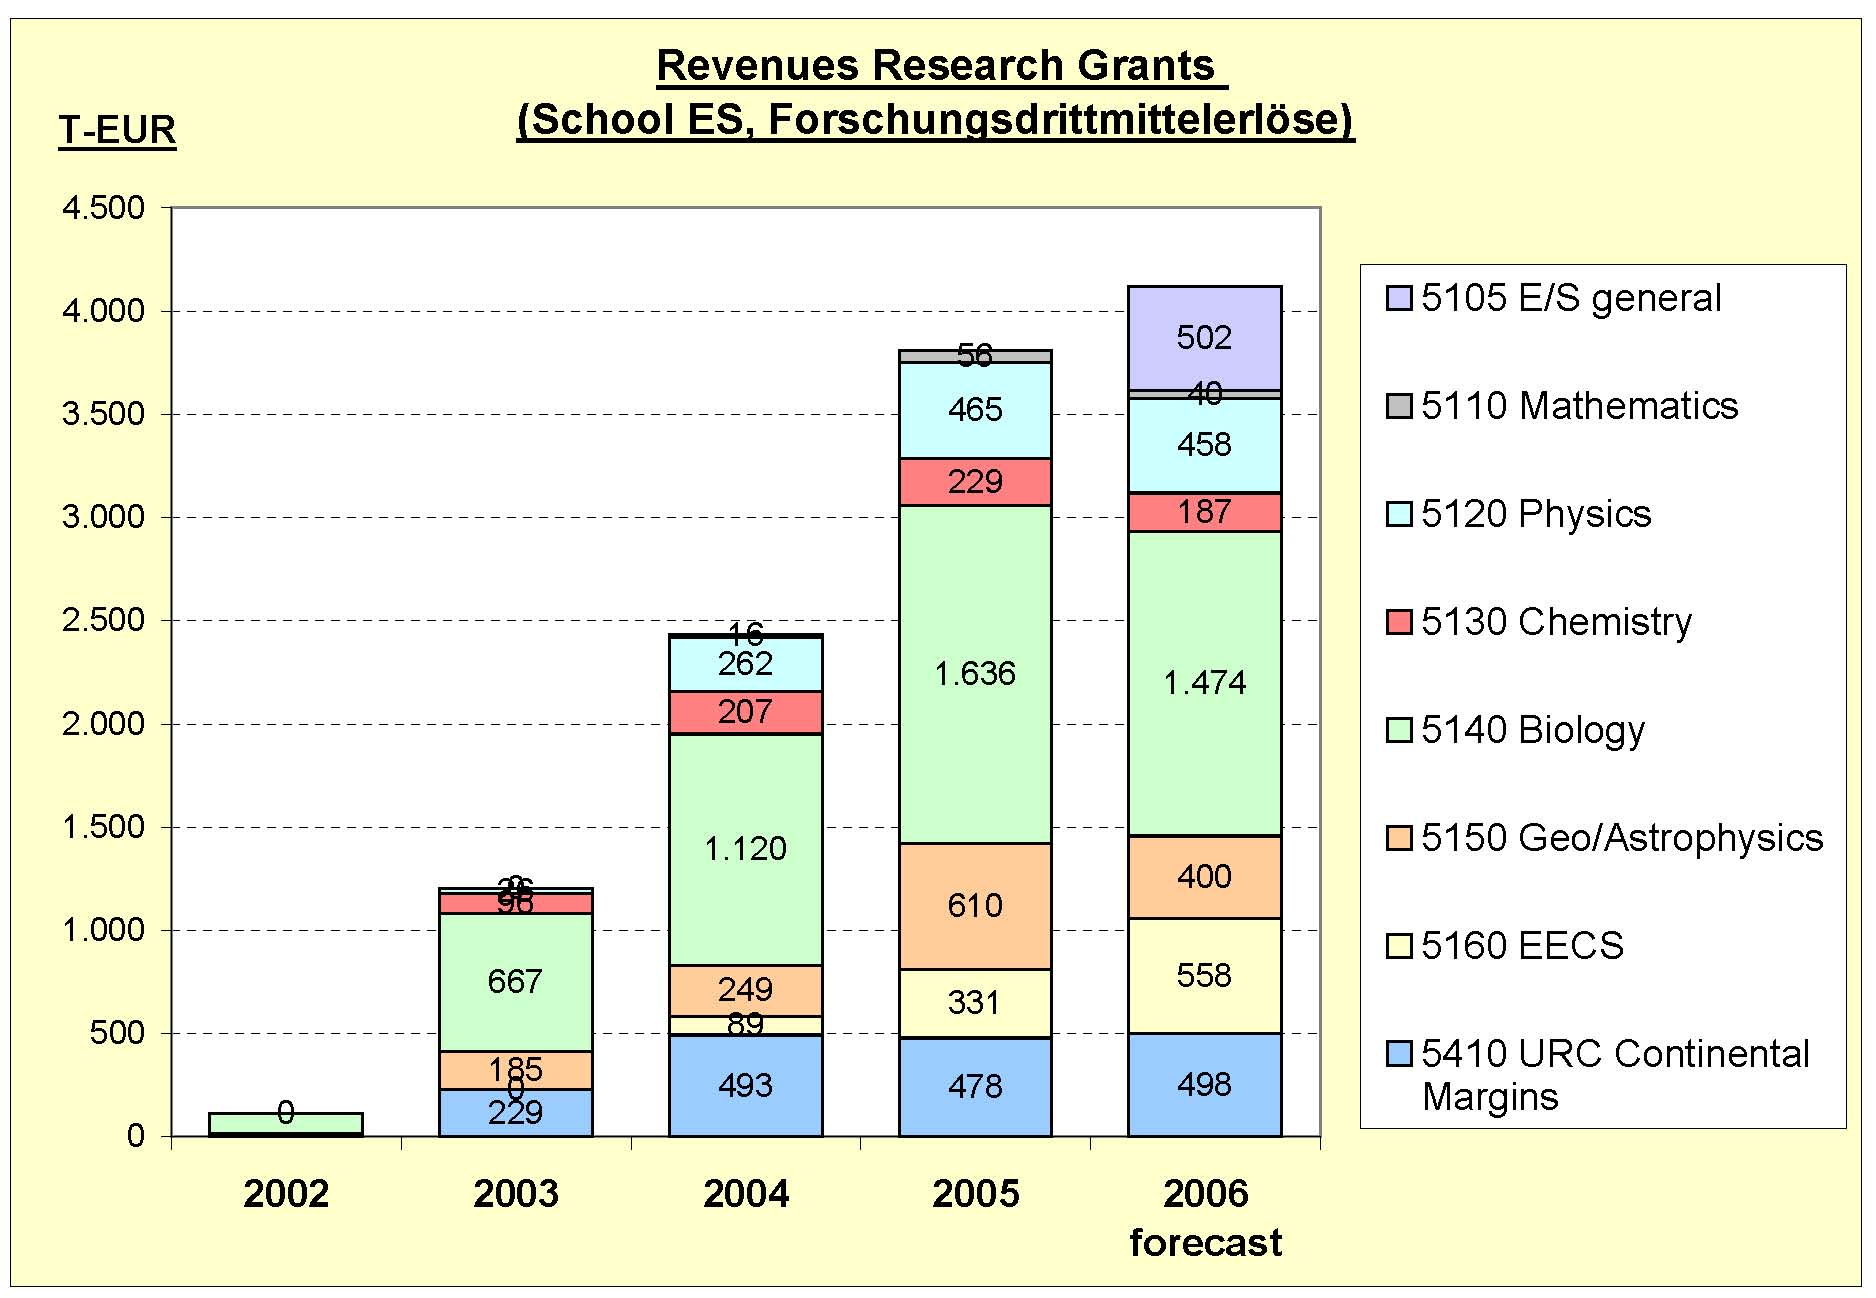
\includegraphics[width=\hsize]{SchoolESGrants-Charts1.jpg}

   \end{center}
 \caption{Revenue from Research Grants
 \label{fig:grants1}}
\end{figure}

\begin{figure}[ht]
  \begin{center}
   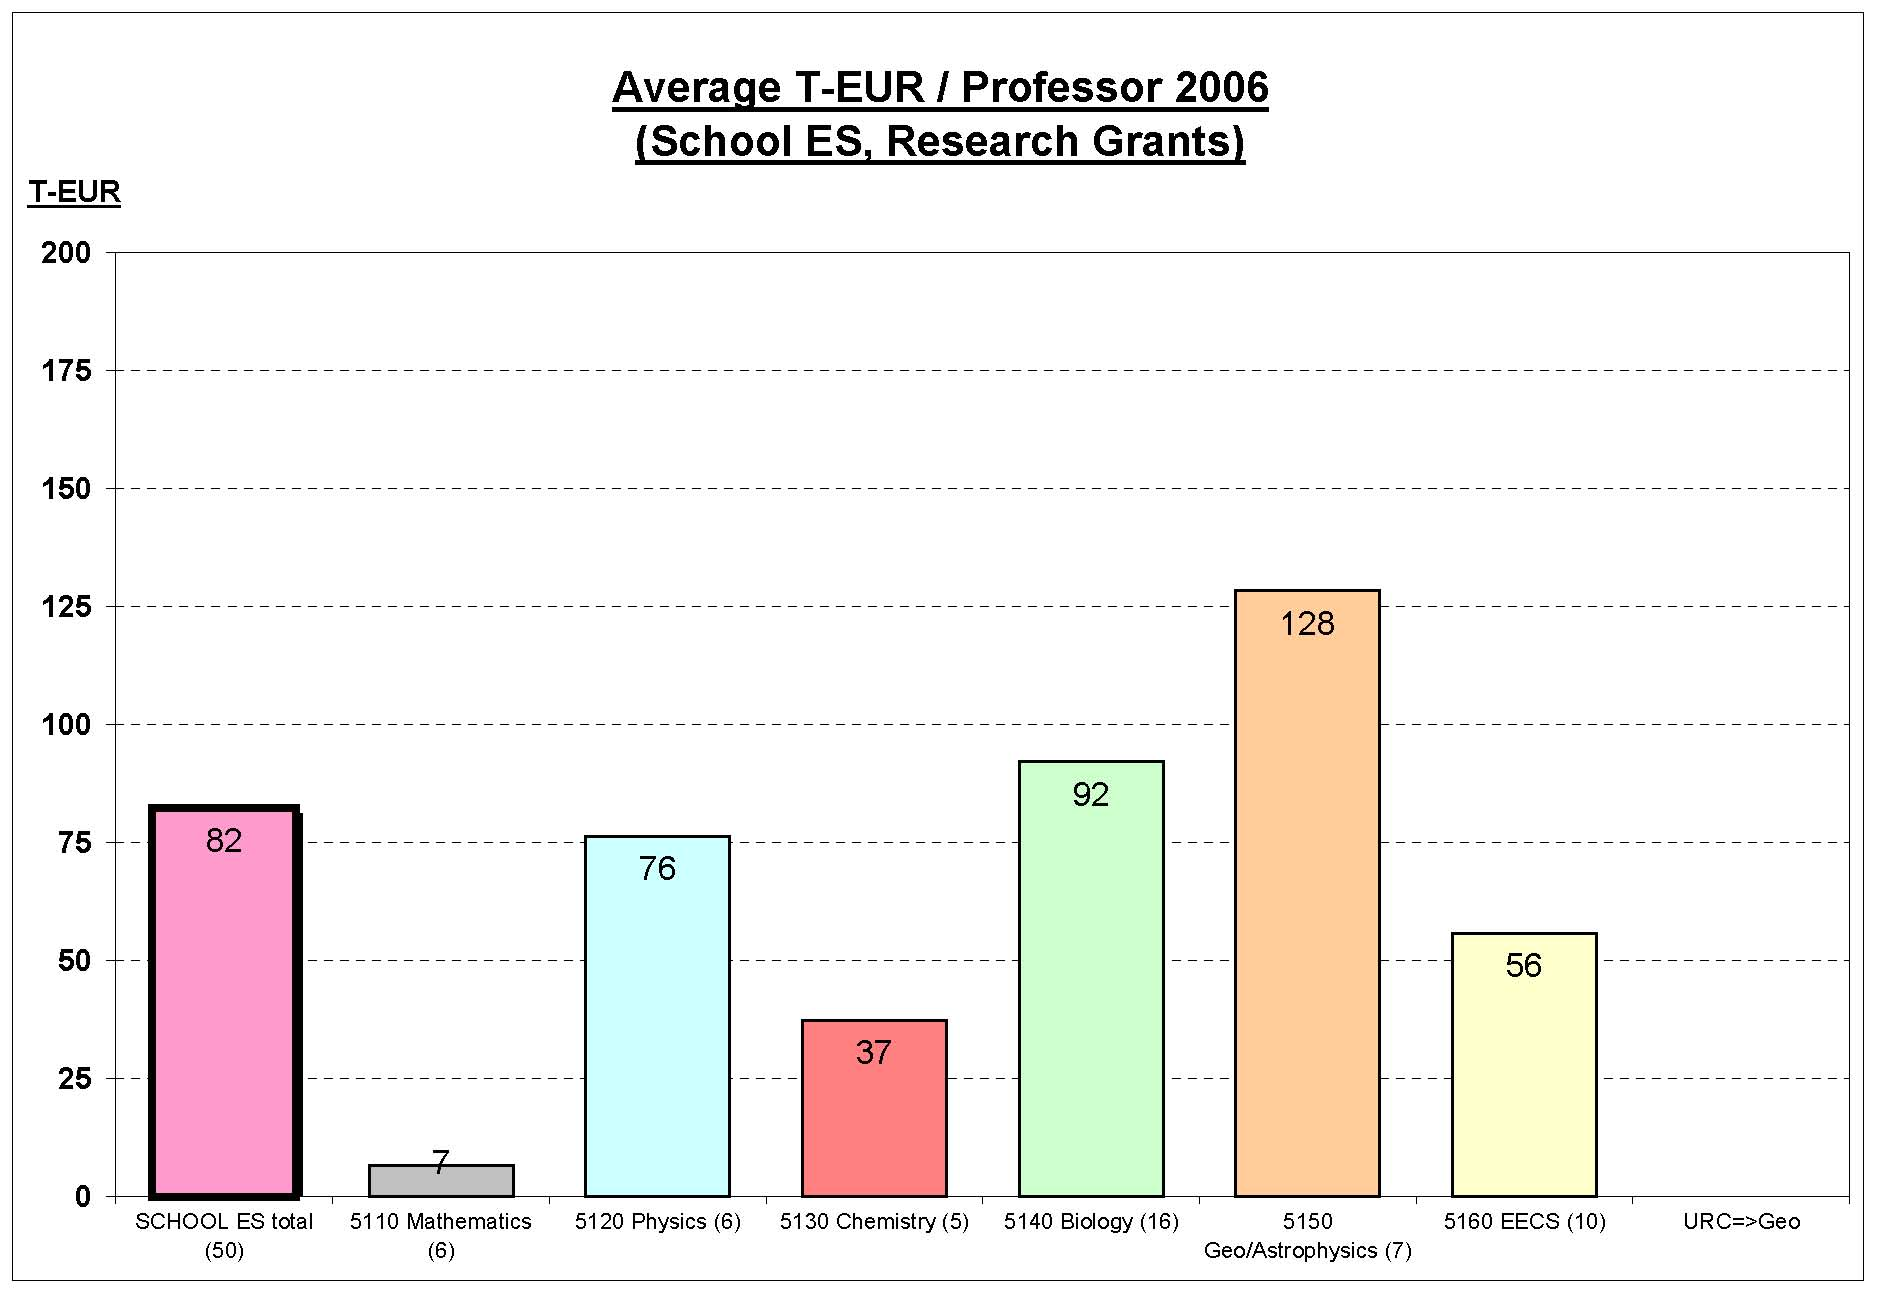
\includegraphics[width=\hsize]{SchoolESGrants-Charts2.jpg}
   \end{center}
 \caption{Research Grants Average T-EUR/Professor
 \label{fig:grants2}}
\end{figure}

\subsection{Personnel} Presently, the School comprises in
total 64 professors out which four are adjunct professors, located
at the Alfred-Wegner-Institut in Bremerhaven. Two distinguished
professors and six university lecturers complete the faculty. In
addition, 70 research associates, five research assistants, 26
technicians, 1 director and 7 assistants belong to the staff. In
2006, several new faculty members have been hired.

\begin{myitemize}
\item Dr. Marc-Thorsten H�tt, Associate Professor of Computational
Systems Biology
 \item   Dr. Ulrich Kleinkath\"ofer, Associate Professor of
Theoretical Physics
\item Dr. Nikolai Kuhnert, Associate Professor of Chemistry
\item  Dr. Lars Linsen,  Associate Professor
of Computational Science and Computer Science
\item   Dr. Bendick Mahleko, University
Lecturer of Computer Science \item Dr. Danilo Roccatano, University
Lecturer of Chemistry
\item  Jon Wallace, PhD, Assistant Professor of
Electrical Engineering \item Dr. Karen Wiltshire, Professor of
Marine Geosciences.
\end{myitemize}

In Mathematics, the visiting professors Prof. Grigori Litvinov and
Prof. Vladimir Tikhomirov, and Dr. Marc Comerford (research
instructor) left. They are replaced by \begin{myitemize} \item  Dr.
Stefan Baier (Visiting Lecturer for Mathematics) \item Kaivan
Mallahi-Karai, PhD (Visiting Lecturer for Mathematics) \item Dr.
Alexei Belov (Visiting Professor for Mathematics).
\end{myitemize}

The following members of the faculty have been promoted during 2006.
\begin{myitemize}
\item  Dr. Klaudia Brix from Associate to Full Professor
\item Dr. Albert Jeltsch from Associate to Full Professor
\item   Dr. Laurenz Thomsen from Associate to Full Professor
\item Marcus Br\"uggen, PhD, from  Assistant to Associate Professor
\item Claus C. Hilgetag, PhD, from Assistant to Associate Professor
\item Dr. Ulrich Schwaneberg from Assistant to Associate Professor.
\end{myitemize}

\null
Dr. Stefano Carpin, Assistant Professor of Computer Science,
has accepted an offer of an Assistant Professorship at University of
California, Merced, USA, starting on January 1, 2007.

\subsection{International Center for Transdisciplinary Science}
 The "International Center for Transdisciplinary Studies"
has been founded and started to operate. The center invites
internationally highly ranked scientists as fellows for periods of
several weeks, mostly during the summer break. The visiting
scientists are generally expected to participate in ongoing
scientific activities. In 2006, 46 scientists have been
participating, among them 39 from foreign countries, see
Section~\ref{ICTS}.

\subsection{Workshops and Summer Schools}

During the year, several international research workshops have been
organized on the campus by members of the faculty.

\begin{myitemize}
\item
From October 19-22, the International Workshop on Astrobiology took
place at IUB, organized by Professor M. Bau.  Focus of the workshop
were Banded Iron Formations (BIFs), that developed between two and
four billion years ago in the precambrian era.  The workshop aimed
at providing an overview on current ideas on the formation and
preservation of Precambrian BIF, on the use of BIF as proxies for
Precambrian seawater, on differences between Early Precambrian BIF
and younger ironstones and hydrogenetic Fe(-Mn) precipitates, and on
experimental set-ups to simulate BIF-related processes in Early
Precambrian environments.

\item
A workshop for young scientists is offered biannually by the DFG
Schwerpunktprogramm SPP1170 (priority program) ''Directed Evolution
to Optimize and Understand Molecular Biocatalysts''. This year's
workshop  took place from July 30 - August 1 on the IUB campus,
organized by Professor U. Schwaneberg. 70 scientists from the 17 DFG
institutions participated in the program.


\item
From July 28 - August 5, a Summer School for students and postdocs
took place. Focus of the more than 50 lectures and workshops has
been on recent research perspectives in biosensing and its
application. 70 participants from 14 Nations met on IUB campus.
 The fourth IUB Summer School has been organized
by Professor M. Winterhalter.


\item In June 2006, the 10th International RoboCup has been organized
in Bremen. More than 400 teams and 2500 participants from 36
countries participated and competed in three main categories: the
robot soccer competition, the robot rescue competition (coordinated
by Professor A. Birk), and the RoboCupJunior for educational
purposes. IUB teams participated in the "Rescue Robot League" and
the "Virtual Robot Competition". The team led by Professor A. Birk
reached the finals of the Robot League and won the Innovation Award,
a student team led by Professor S. Carpin came in second place in
the Virtual Robot Competition.

\item
From January 16-20, IUB  hosted the international "HERMES Graduate
Training and Job Fair". More than 30 Master's and PhD students
working at HERMES partner institutions all over Europe participated.
The HERMES (Hotspot Ecosystem Research on the Margins of European
Seas) Program, funded by the European Commission, was begun to gain
better understanding of life in depths of between 200 and 2000
meters and deeper.

\end{myitemize}


\subsection{Research Highlights}

Researchers of the School of Engineering and Science have been
contributing towards the international scientific progress with
several important discoveries that have been published in the most
prestigious international journals.

\begin{myitemize}
\item
Pofessor A. Jeltsch and his co-workers from IUB, the Institute of
Biochemistry of the University of Giessen, and the Medical Research
Council of Cambridge University (UK) for the first time successfully
used genetically engineered proteins to deactivate Herpes viruses in
human cell lines. The study is published in the November 2006 issue
of Nucleic Acids Research

\item
Professor S. Tautz and his group for the first time managed to
detect a much larger delocalization of electrons in an organic
monolayer semiconductor deposited on a metallic substrate than ever
detected in an insulated organic semiconductor. The results, which
were published in Nature 444, p. 350 - 353, on November 16, 2006,
allow insights into basic mechanisms of electron transport within
organic materials and their interfaces with metallic surfaces.

\item
On the 68th cruise of the German research vessel METEOR an
international team of scientists under the lead of Professor A.
Koschinsky registered 407 $^{\circ}$ C at a hydrothermal vent as the
highest temperature on record measured at the ocean bottom (May 22,
2006).  The scientists registered the record temperature in 3000m
water depth at a so-called ''black smoker'', a hydrothermal deep-sea
vent with a characteristic particle plume in the discharge water.
Maximum deep-sea water temperatures up to 402 $^{\circ}$C so far
have only been observed in the Pacific.




\item
Professor S. Rosswog and D. Price, Postdoc at the University of
Exeter, for the first time were able to demonstrate in supercomputer
simulation of a neutron star merger that a collision of these super
dense cosmic objects create magnetic fields a quadrillion
(10$^{15}$) times stronger than the magnetic field of the earth. The
simulation results are published in the online express issue of
Science ("Producing ultra-strong magnetic fields in magnetized
neutron star mergers").

\item
Professor C. Hilgetag and his colleague H. Barbas, Professor of
Health Sciences at Boston University, found new answers to one of
the oldest questions in neuroscience: How do the characteristic
folds of the primate brain cortex form? The results of an extensive
analysis of neuroanatomic data are published as the cover story in
the PLoS Computational Biology ("Role of Mechanical Factors in the
Morphology of the Primate Cerebral Cortex", Volume 2, Issue 3, MARCH
2006, www.ploscompbiol.org). Prof. C. Hilgetag for the first time
was able to provide empirical evidence for the hypothesis that the
characteristic folds of the primate brain are mainly formed by
mechanical forces of fiber tension.


\end{myitemize}


\subsection{Noteworthy}
\begin{myitemize}
\item
On November 15,  the association Unifreunde e. V. awarded the Ernst
A. C. Lange Prize for the joint research project ''New display
technology for mobile applications" of IUB and University of Bremen.
The award, which is endowed with 5000 euros prize money,
acknowledges innovative co-operational research between scientists
of the two Bremen universities in the fields of Mathematics, Natural
and Technical Sciences. The two laureates 2006 are the two Bremen
scientists Professor D. Knipp and Professor W. Benecke, Professor of
Physics, Electronics and Information Technology at University of
Bremen.


\item Researchers from all over Germany were taking part in the Science
Festival "Highlights of Physics" from  November 6-10  in Bremen.
Under the motto of "WaveWorlds" scientists gave an introduction into
wave phenomena in water, light and sound through series of talks,
live experiments and science shows.  IUB was involved in the
organization and preparation of this event. Faculty and staff
contributed in particular to the big opening show, the exhibition,
and the physics competition for pupils.

\item
In October the research network International Research Consortium on
Continental Margins (IRCCM) under IUB's lead started a new research
project on biomonitoring of cold water coral reefs in the vicinity
of oil exploration sites. The aim of the 1.2 million euro project
financed by the Norwegian company Statoil is to develop new
monitoring and ecosystem modelling approaches for risk assessment in
the off-shore industry.  Research site is the Tisler cold water
coral reef in the Skagerrak, which was placed under environmental
protection by the Norwegian government in 2003. It will host IUB's
second deep-sea online observatory.


\item
On April 23,  IUB's RoboCup team managed another international
tournament victory at the US Open Robot Rescue League in Atlanta,
prevailing against the other competing institutions only two weeks
after their success at the Dutch Open in Eindhoven. The ten
contesting teams in Atlanta included such renowned institutions as
the Georgia Institute of Technology and Carnegie Mellon University,
which demonstrated with their impressive investments into their
teams the importance of research on search and rescue robots in the
US.

\item
Informatics Year has being organised in conjunction with the Science
in Dialogue initiative and the Gesellschaft f�r Informatik (GI) as
well as with numerous partners in the fields of science, industry
and culture. The idea behind this Science Year was to familiarise a
broader public with the contents, processes and practical
applications of science and to do so in an informative, exciting and
entertaining way. IUB was involved in exhibitions, the Symposium on
Artificial Intelligence and various other activities.

\end{myitemize}
\ \ \\
\ \ \\

Bremen, January 2007


\begin{figure}[ht]
     
\includegraphics[width=4cm]{DeanSig}
 \end{figure}



Prof. Dr.~Dr.~h.c.~Bernhard Kramer \\
Vice President and Dean \\
School of Engineering and Science
